\chapter{Implementation}
\label{cap5}



\section{Graphical editor}\label{editor}

Description of the GEF Framework with code examples
\\
Graphical Editing Framework (GEF) provides a powerful foundation for creating editors for visual editing of arbitrary models. Its effectiveness lies in a modular build, fitting use of design patterns, and decoupling of components that comprise a full, working editor. To a newcomer, the sheer number and variety of concepts and techniques present in GEF may feel intimidating. However, once learned and correctly used, they help to develop highly scalable and easy to maintain software. This section aims to provide a gentle yet comprehensive introduction to GEF. It describes our Pluto Graphical Editor.


\section{Code generation}\label{codeGeneration}

Description of the generation process of the code from diagram

\section{Object-oriented approach}\label{oomodel}

Why we decided to use JAVA, How we implement entities, UML diagrams of classes, MVC pattern

\section{Runtime Management}\label{runtimeMng}

Description of the management of threads, pub/sub pattern and log procedures

\section{User interface}\label{interface}

We chose the Swing tool to develop the Pluto User Interface, already described in section \ref{plutoMainApp}.
We made this choice since Swing is well known to us.
Indeed we used it for the development of many academic projects, where we noticed that it allows to build graphical interface in a very fast and easy way and to add a great variety of components.
\\

Swing library is an official Java GUI toolkit released by Sun Microsystems. It is used to create Graphical user interfaces with Java.
The main characteristics of the Swing toolkit:
\begin{itemize}
\item platform independent
\item customizable
\item extensible
\item configurable
\item lightweight
\end{itemize}

Swing is an advanced GUI toolkit. It has a rich set of widgets. From basic widgets like buttons, labels, scrollbars to advanced widgets like trees and tables. Swing itself is written in Java.
Swing is a part of JFC, Java Foundation Classes. It is a collection of packages for creating full featured desktop applications.

There are basically two types of widget toolkits: \textit{Lightweight} and \textit{Heavyweight}.
A heavyweight toolkit uses OS's API to draw the widgets. For example Borland's VCL is a heavyweight toolkit since it depends on WIN32 API, the built in Windows application programming interface.
As already said, Swing is a lightweight toolkit since it paints its own widgets.

\section{The crazyflie nano-quadcopter}\label{crazyflie}

For the concrete actuation of the sensing tasks required by each application, we chose the Crazyflie Nano-Quadcopter, shown in figure \ref{fig:crazyflie}.


\begin{figure}[H]
\centering
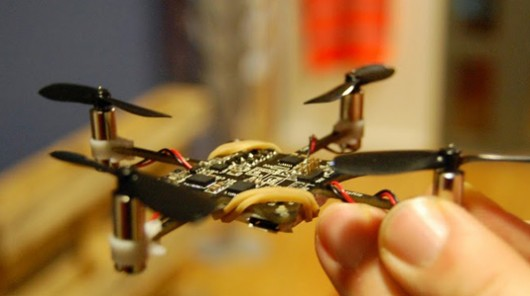
\includegraphics[width=\linewidth]
{pictures/crazyflie.jpg}
  \caption{The Crazyflie Nano-Quadcopter}
  \label{fig:crazyflie}
\end{figure}

The Crazyflie is a tiny quadcopter often referred to as a nano-quad, built using the PCB itself as the frame,developed solely by open source tools. The Crazyflie specs are the following:


\begin{itemize}
\item {Small and lightweight, around 19g and about 90mm motor to motor
}
\item {Flight time up to 7 minutes with standard 170mAh Li-Po battery
}
\item {Standard micro-USB connector for charging which takes 20min for the stock 170mAh Li-Po battery
}
\item {On-board low-energy radio@1mW based on the nRF24L01+ chip. Up to 80m range (environment dependent) when using the Crazyradio USB dongle}
\item{Radio bootloader which enables wireless update of the firmware
}
\item{Powerful 32 bit MCU: STM32F103CB @ 72 MHz (128kb flash, 20kb RAM)
}
\item{3-axis high-performance MEMs gyros with 3-axis accelerometer: Invensense MPU-6050
}
\item{Available footprints to manually solder magnetometer HMC5883L/HMC5983 or/and barometer MS5611
}
\item{4-layer low noise PCB design with separate voltage regulators for digital and analog supply
}
\end{itemize}

To concretely control the Crazyflie, there is a Python library which gives high level functions and hides the details.
We used a particular API to send the control command: 
\\

\begin{lstlisting}
	send_setpoint(roll, pitch, yaw, thrust)
\end{lstlisting}

The arguments roll/pitch/yaw/trust is the new set-points that should be sent to the copter.
Foe example, to send a new control set-point:
\\

\begin{lstlisting}
	roll    = 0.0
    pitch   = 0.0
    yawrate = 0
    thrust  = 0
    crazyflie.commander.send_setpoint(roll, pitch, yawrate, thrust)
\end{lstlisting}

Changing the \textit{roll} and \textit{pitch} will make the quadcopter tilt to the sides and thus change the direction that it's moving in.
Changing the \textit{yaw} will make the quadcopter spin.
The thrust is used to control the altitude of the quadcopter.

By dynamically adjusting these four parameters we can make the Crazyflies move to the user specified locations.


